\documentclass{article}

% if you need to pass options to natbib, use, e.g.:
% \PassOptionsToPackage{numbers, compress}{natbib}
% before loading nips_2017
%
% to avoid loading the natbib package, add option nonatbib:
% \usepackage[nonatbib]{nips_2017}

%\usepackage{nips_2017}

% to compile a camera-ready version, add the [final] option, e.g.:
\usepackage{nips_2017}

\usepackage[utf8]{inputenc} % allow utf-8 input
\usepackage[T1]{fontenc}    % use 8-bit T1 fonts
\usepackage{hyperref}       % hyperlinks
\usepackage{url}            % simple URL typesetting
\usepackage{booktabs}       % professional-quality tables
\usepackage{amsfonts}       % blackboard math symbols
\usepackage{nicefrac}       % compact symbols for 1/2, etc.
\usepackage{microtype}      % microtypography
\usepackage{graphicx}
\usepackage{caption}
\usepackage{subcaption}

\title{Time Domain Neural Audio Style Transfer}

% The \author macro works with any number of authors. There are two
% commands used to separate the names and addresses of multiple
% authors: \And and \AND.
%
% Using \And between authors leaves it to LaTeX to determine where to
% break the lines. Using \AND forces a line break at that point. So,
% if LaTeX puts 3 of 4 authors names on the first line, and the last
% on the second line, try using \AND instead of \And before the third
% author name.

\author{
  Parag K. Mital\\
  Kadenze, Inc.\thanks{http://kadenze.com}\\
  \texttt{parag@kadenze.com} \\
  %% examples of more authors
  %% \And
  %% Coauthor \\
  %% Affiliation \\
  %% Address \\
  %% \texttt{email} \\
  %% \AND
  %% Coauthor \\
  %% Affiliation \\
  %% Address \\
  %% \texttt{email} \\
  %% \And
  %% Coauthor \\
  %% Affiliation \\
  %% Address \\
  %% \texttt{email} \\
  %% \And
  %% Coauthor \\
  %% Affiliation \\
  %% Address \\
  %% \texttt{email} \\
}

\begin{document}
% \nipsfinalcopy is no longer used

\maketitle

\begin{abstract}
  A recently published method for audio style transfer has shown how to extend the process of image style transfer to audio.  This method synthesizes audio "content" and "style" independently using the magnitudes of a short time Fourier transform, shallow convolutional networks with randomly initialized filters, and iterative phase reconstruction with Griffin-Lim.  In this work, we explore whether it is possible to directly optimize a time domain audio signal, removing the process of phase reconstruction and opening up possibilities for real-time applications and higher quality syntheses.  We explore a variety of style transfer processes on neural networks that operate directly on time domain audio signals and demonstrate one such network capable of audio stylization.
\end{abstract}

\section{Introduction}

% Style transfer \cite{} is a method for optimizing a randomly initialized image to have the appearance of the content and style of two separate images.  It works by finding the raw activations of a so-called "content" image and optimizing a noise image to resemble the same activations while for "style", it looks at the kernel activations of any given layer and optimizes for these.  The original work by Gatys et al. demonstrated this technique using activations from pre-trained VGG deep convolutional networks, though recent techniques in texture synthesis \cite{} show that similar results are possible with randomly initialized shallow convolutional networks.

Audio style transfer \cite{Ulyanov2016} attempts to extend the technique of image style transfer \cite{Gatys} to the domain of audio, allowing "content" and "style" to be independently manipulated.  Ulyanov et al. demonstrates the process using the magnitudes of a short time Fourier transform representation of an audio signal as the input to a shallow untrained neural network, following similar work in image style transfer \cite{Ulyanov2016b}, storing the activations of the content and Gram activations of the style.  A noisy input short time magnitude spectra is then optimized such that its activations through the same network resemble the target content and style magnitude's activations.  The optimized magnitudes are then inverted back to an audio signal using an iterative Griffin-lim phase reconstruction process \cite{Griffin1984}.

Using phase reconstruction ultimately means the stylization process is not modeling the audio signal's fine temporal characteristics contained in its phase information.  For instance, if a particular content or style audio source were to contain information about vibrato or the spatial movement or position of the audio source, this would likely be lost in a magnitude-only representation.  Further, by relying on phase reconstruction, some error during the phase reconstruction is likely to happen, and developing real-time applications are also more difficult \cite{Wyse2017}, though not impossible \cite{Prusa2017}.  In any case, any networks which discard phase information, such as \cite{Wyse2017}, which build on Ulyanov's approach, or recent audio networks such as \cite{Hershey2016} will still require phase reconstruction for stylization/synthesis applications.

Rather than approach stylization/synthesis via phase reconstruction, this work attempts to directly optimize a raw audio signal.  Recent work in Neural Audio Synthesis has shown it is possible to take as input a raw audio signal and apply blending of musical notes in a neural embedding space on a trained WaveNet autoencoder \cite{Engel2017}.  Though their work is capable of synthesizing raw audio from its embedding space, there is no separation of content and style using this approach, and thus they cannot be independently manipulated.  However, to date, it is not clear whether this network's encoder or decoder could be used for audio stylization using the approach of Ulyanov/Gatys.

To understand better whether it is possible to perform audio stylization in the time domain, we investigate a variety of networks which take a time domain audio signal as input to their network: using the real and imaginary components of a Discrete Fourier Transform (DFT); using the magnitude and unwrapped phase differential components of a DFT; using combinations of real, imaginary, magnitude, and phase components; using the activations of a pre-trained WaveNet decoder \cite{Oord2016b,Engel2017}; and using the activations of a pre-trained NSynth encoder \cite{Engel2017}.  We then apply audio stylization similarly to Ulyanov using a variety of parameters and report our results.

% \section{Related Work}

% There have been a few investigations of audio style transfer employing magnitude representations, such as Ulyanov's original work and a follow-up work employing VGG \cite{Wyse2017}.  These models discard the phase information in favor of phase reconstruction.  As well, there have been further developments in neural networks capable of large scale audio classification such as \cite{Hershey2016}, though these are trained on magnitude representations and would also require phase reconstruction as part of a stylization process.  Perhaps most closely aligned is the work of NSynth \cite{Engel2017}, whose work is capable of taking as input a raw audio signal and allows for applications such as the blending of musical notes in a neural embedding space.  Though their work is capable of synthesizing raw audio from its embedding space, there is no separation of content and style, and thus they cannot be independently manipulated.

% Speech synthesis techniques
%TacoTron demonstrated a technique using ... 
%In a similar vein, WaveNet, ... 
%NSynth incorporates a WaveNet decoder and includes an additional encoder, allowing one to encode a time domain audio signal using the encoding part of the network with 16 channels at 125x compression, and use these as biases during the WaveNet decoding.  The embedding space is capable of linearly mixing instruments in its embedding space, though has yet to be explored as a network for audio stylization where content and style are indepenently manipulated.

% SampleRNN

% Soundnet

% VGG (Lonce Wyse, https://arxiv.org/pdf/1706.09559.pdf); 

% Zdenek Pruska

% Other networks exploring audio include VGGish, built on the AudioSet dataset.  This network, like Ulyanov's original implementation, however does not operate on the raw time domain signal and would require phase reconstruction.  However, it does afford a potentially richer representation than a shallow convolutional network, as its embedding space was trained with the knowledge of many semantic classes of sounds.

% CycleGAN (https://gauthamzz.github.io/2017/09/23/AudioStyleTransfer/)


\section{Experiments\footnote{Further details are described in the Supplementary Materials}}

We explore a variety of computational graphs which use as their first operation a discrete Fourier transform in order to project an audio signal into its real and imaginary components.  We then explore manipulations on these components, including directly applying convolutional layers, or undergoing an additional transformation of the typical magnitude and phase components, as well as combinations of each these components.  For representing phase, we also explored using the original phase, the phase differential, and the unwrapped phase differentials.  From here, we apply the same techniques for stylization as described in \cite{Ulyanov2016}, except we no longer have to optimize a noisy magnitude input, and can instead optimize a time domain signal.  We also explore combinations of using content/style layers following the initial projections and after fully connected layers.

We also explore two pre-trained networks: a pre-trained WaveNet decoder, and the encoder portion of an NSynth network as provided by Magenta \cite{Engel2017}, and look at the activations of each of these networks at different layers, much like the original image style networks did with VGG.  We also include Ulyanov's original network as a baseline, and report our results as seen through spectrograms and through listening.  Our code is also available online\footnote{https://github.com/pkmital/neural-audio-style-transfer}.

\section{Results}

Only one network was capable of producing meaningful audio reconstruction through a stylization process where both the style and content appeared to be retained: including the real, imaginary, and magnitude information as concatenated features in height and using a kernel size 3 height convolutional filter.  This process also includes a content layer which includes the concatenated features before any linear layer, and a style layer which is simply the magnitudes, and then uses a content and style layer following each nonlinearity.  This network produces distinctly different stylizations to Ulyanov's original network, despite having similar parameters, often including quicker and busier temporal changes in content and style.  The stylization also tends to produce what seems like higher fidelity syntheses, especially in lower frequencies, despite having the same sample rate.  Lastly, this approach also tends to produce much less noise than Ulyanov's approach, most likely due to errors in the phase reconstruction/lack of phase representation.

Every other combination of input manipulations we tried tended towards a white noise signal and did not appear to drop in loss.  The only other network that appeared to produce something recognizable, though with considerable noise was using the magnitude and unwrapped phase differential information with a kernel size 2 height convolutional filter.  We could not manage to stylize any meaningful sounding synthesis using the activations in a WaveNet decoder or NSynth encoder.

% VGGish, AudioSet; VGG equivalent for audio, but uses a log-mel spectrogram.

\section{Discussion and Conclusion}

This work explores neural audio style transfer of a time domain audio signal.  Of these networks, only two produced any meaningful results: the magnitude and unwrapped phase network, which produced distinctly noisier syntheses, and the real, imaginary, and magnitude network which was capable of resembling both the content and style sources in a similar quality to Ulyanov's original approach, though with interesting differences.  It was especially surprising that we were unable to stylize with NSynth's encoder or decoder, though this is perhaps to due to the limited number of combinations of layers and possible activations we explored, and is worth exploring more in the future.

% Style transfer, like deep dream and its predecessor works in visualizing gradient activations, through exploration have the potential to enable us to understand representations created by neural networks.  Through synthesis, and exploring the representations at each level of a neural network, we can start to gain insights into what sorts of representations if any are created by a network.  However, to date, very few explorations of audio networks for the purpose of dreaming or stylization have been done.  

%End to end learning, http://www.mirlab.org/conference_papers/International_Conference/ICASSP\%202014/papers/p7014-dieleman.pdf - spectrums still do better than raw audio.

\small
\bibliographystyle{IEEEtran}
\bibliography{style-transfer}

\section{Supplementary Material}

\subsection{Input Data}

Each of the shallow untrained networks we used take as input a raw audio signal sampled at 22050 Hz with a frame size of 2048 samples, an alpha of 0.01, and use 150 iterations of the Adam optimizer.  We explored manipulations in sample rate including [44100, 22050, and 16000].  For frame size (DFT size was always set to half frame size with no padding or centering), we explored [1024, 2048, 4096, 8192], with hop sizes of [128, 256, 512].  The resulting projections from a discrete Fourier basis set were then sliced to half width to remove their symmetric projections.

For the NSynth and WaveNet networks, we used the native sampling rate they were trained on, 16000 Hz.  For the shallow untrained networks, we explored a combination of networks that varied in their initial input processing, depth, and the number layers and information we used for content and stylization.  We tested networks which incorporated the real, imaginary, magnitude, and phase information of an audio source signal's DFT, as computed with a computational graph capable of automatic differentiation.  This enabled us to apply stylization by optimizing an input noise signal, while keeping the rest of the network untrained.

\subsection{Network}

Ulyanov's original stylization network uses depth-wise convolution as the first layer operating on the magnitudes.  We employ the same technique here, except using combinations of the real, imaginary, magnitude, and phase information as input, stacked along the height dimension.  For kernel sizes, we tried a variety of widths, including ${[4, 8, 16]}$, and for heights, depending on the number of components included we tried ${[1, H]}$, where $H$ is the total number of components included in the model.  For instance, for a model incorporating real and imaginary components, we set $H = 2$, and stacked the real and imaginary comopnents in rows. For number of layers, we tried ${[1, 2, 3]}$.  And finally, for representing phase, we tried the original phase, the phase differential, and the unwrapped phase differentials.  We used a stride of 1 and a ReLu activation for all convolutional layers, and followed the weight initialization used by Ulyanov's baseline audio stylization network.  Finally, we explored alphas including [0.1, 0.05, 0.01, 0.005, 0.001, 0.0005, 0.0001].

\begin{figure}
\centering
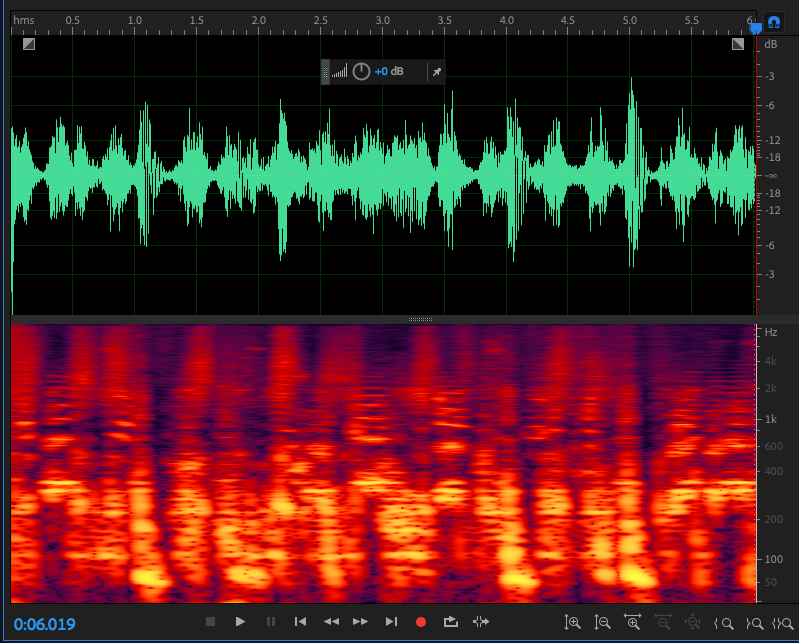
\includegraphics[width=1\linewidth]{synthesis}
\caption{Example synthesis optimizing audio directly with both the source content and style audible.}
\end{figure}
\end{document}
